

\section{Ponteiros}

\begin{frame}[allowframebreaks=0.7]


\frametitle{\Large Capítulo xxxxx -- Ponteiros}
\begin{columns}
\begin{column}{.4\textwidth}
\centering
Pontos fundamentais a serem cobertos:
  
  \begin{small}
  \begin{enumerate}
  \item \textbf{\textcolor{red}{Pré-requisito: prática na linguagem C}}
  \item Uso de Memória
  \item Alocação de memória Estática x Dinâmica
  \item Alocação dinâmica de memória
  \item  Funções para alocação de memória
  \item  Utilizando as funções para alocação de memória
  \item  Alocação de memória e estruturas em C
  \item  Ponteiros para ponteiros
  \item Mais alocação de vetores e matrizes como ponteiros
\end{enumerate}  
  \end{small}
  
\end{column}

\begin{column}{.6\textwidth}
%\centering
%\vspace{-2cm}
\vskip -1.5cm

\includegraphics[height=6cm, width=7cm]{figs/fig_ponteiros/null-pointer.png}
%\hspace{+0.25cm}
%\scriptsize\textcolor{red}{[Tizio, Caio et al., Nature (2006)]}
\end{column}

\end{columns}

\end{frame}



\begin{frame}[allowframebreaks=0.9]

\frametitle{Motivação aos Ponteiros}
\begin{figure}[ht]
  \begin{center}

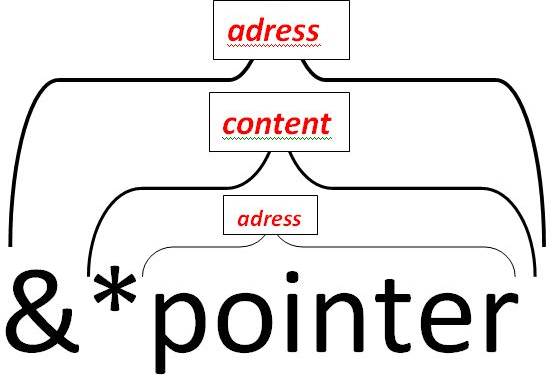
\includegraphics[height=5cm, width=5cm]{figs/fig_ponteiros/hierarq_pointer.png}

    \caption{A história está por vir ...}
 %   \label{fig:}
  \end{center}
\end{figure}

\end{frame}

%------------
